\section{国内外研究现状及难点}
\label{sec:intro:background}

%本节说了什么
在不同的应用场景中,已经有多种时间隐通道构造方法,不同的方法在原理及特性方面存在差异。
%本节包含的内容
本节主要介绍移动互联网中时间隐通道的发展现状,以及时间隐通道的鲁棒性策略,最后介绍常用的时间隐通道检测方法。

\subsection{隐通道分类及特征}
\label{sec:intro:background:covert-channel}

\insertFigure{
	\begin{figure}[htbp]
        \centering
        \subfigure[基于单主机的隐通道示意图]{
            \label{fig:1:modes:host}
            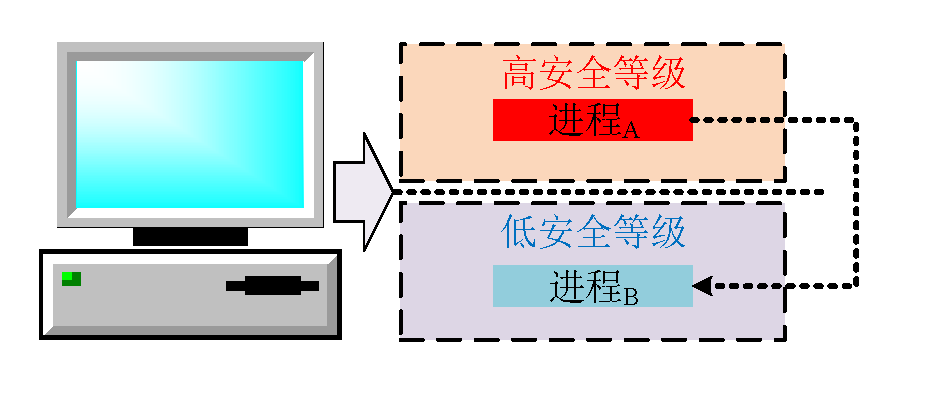
\includegraphics[width=0.48\textwidth]{chapters/chapter1/figures/single-host.pdf}
        }
        \subfigure[基于网络的隐通道示意图]{
            \label{fig:1:modes:net}
            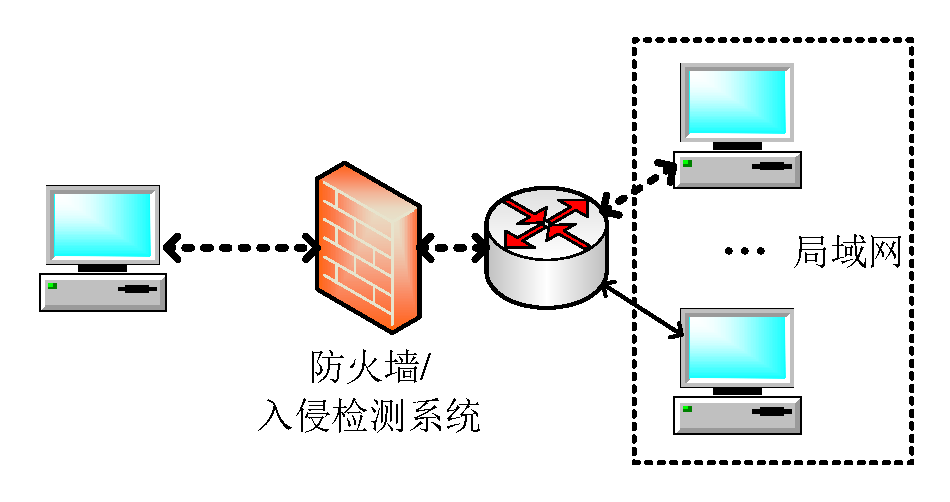
\includegraphics[width=0.48\textwidth]{chapters/chapter1/figures/net-based.pdf}
        }
        \caption{不同环境中的隐通道示意图}
        \label{fig:1:modes}
    \end{figure}
}

根据基本传输原理,隐通道被划分为时间隐通道及存储隐通道。在传输原理方面,存储隐通道的基本方式,是将隐蔽消息写入双方共享的存储位置;时间隐通道基于传输过程的时间特征,将隐蔽消息调制到传输特征中。通过判断原始数据是否被修改,是辨别时间隐通道及存储隐通道的基本方式。因此,对于监听者,判断数据有效性是必要操作。\nupcite{4317620,Cabuk:2004:ICT:1030083.1030108}如图\nref{fig:1:modes},隐通道的应用环境划分为单主机环境及网络环境,单主机平台中隐通道的重点是突破安全软件的限制,将高安全级别的数据泄露给低安全级别的进程。而在网络环境中,隐通道的目标是隐蔽消息在实体之间传输,侧重于突破网络防火墙及审计系统等安全组件。

云计算环境是一种特殊的单主机环境,不同用户的数据及进程虽然已经进行隔离,但仍然保持相同的处理器执行环境,隐通道主要用于突破云计算的进程隔离。借助内存及Cache的共享模式,公有云下的隐通道打破了进程对数据访问的限制,能够突破网络隔离及存储隔离。\nupcite{7368307,6008721,6980363,6744676,7310718,8997733,6832320,8253984,6878465}

随着网络应用范围扩大,网络环境中的隐通道是当前主要研究要点。\nupcite{10.1007/11767831_10,4317620,4630112}在网络环境中,时间隐通道的构建基础为数据包流。存储隐通道可以利用TCP包头中的冗余字段,如序列号字段,进行隐蔽消息传输。\nupcite{5579643}对应的,监听者或防守方通过数据覆写,或者规范化来破坏存储隐通道。\nupcite{7087183,10.1007/11767831_10}对于VoIP等应用,数据发送频率高,基于数据内容的存储隐通道具有较高的性能。\nupcite{8817935,mazurczyk2016youskyde}结合隐写术等数据嵌入方式,存储隐通道在视频及多媒体应用中也具有较好效果。\nupcite{mazurczyk2016youskyde,li2019a}

不同于存储隐通道,时间隐通道基于数据包传输特征,对数据内容不产生任何影响。因此,当监听者进行数据内容审查时,时间隐通道无暴露风险。时间隐通道在传输特征方面,与宿主信道基本一致。监听者审查数据内容或检测传输特征,均无法识别时间隐通道。因此,时间隐通道通过逼近宿主信道的传输特征,具有极佳的隐蔽性,适用严格隐蔽性要求的场景。\nupcite{7299946,8447997}

\subsection{基于移动互联网的时间隐通道}
\label{sec:intro:background:ctc}

%在移动互联网环境下,构建时间隐通道,应当遵守怎样的约束
对于时间隐通道的最基本要求,是传输过程的隐蔽性,并且能够抵御监听者的分析与防御。如图\nref{fig:1:covert-channel},监听者对Alice及Bob的传输内容进行监听与分析,通过分析传输特征的差异识别隐蔽信道。对于监听者,特定的观测对象,一定属于隐蔽信道和宿主信道中的一种。依据宿主信道传输特征的先验知识,判断当前检测到的特征与先验知识的差异,是监听者鉴别时间隐通道的基本方法。

根据常见的时间隐通道构造方法,可检测的传输特征包括IPD、数据包长度以及数据包发送顺序。满足抗检测性约束的时间隐通道方案,应当与宿主信道保持分布一致性。在移动互联网中,传输过程受网络噪声及空口传输干扰,时间隐通道产生误码的概率较高。因此,时间隐通道在设计中应当考虑检错及纠错能力,保证传输可靠性。

%常用的构建方法
\insertFigure{
	\begin{figure}[htbp]
		\centering
        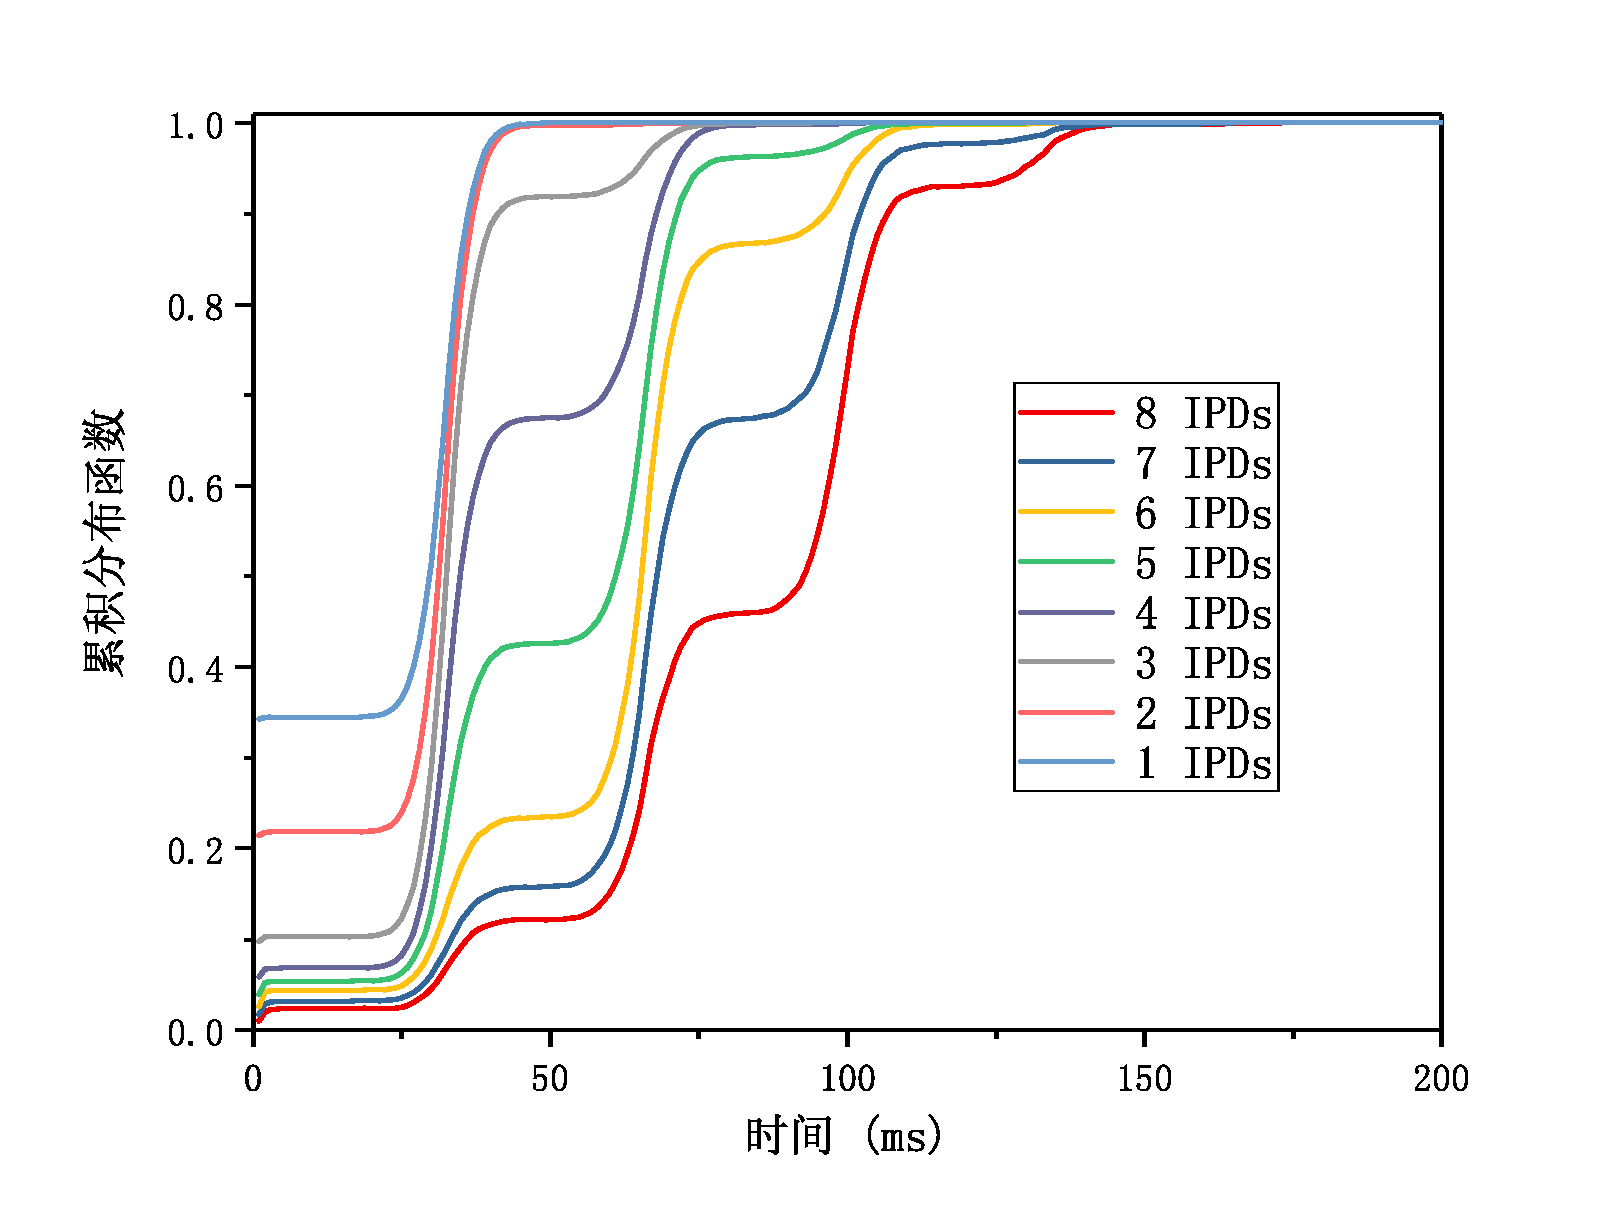
\includegraphics[width=0.75\textwidth]{chapters/chapter1/figures/m-ipds.pdf}
        \caption{VoLTE场景中m-IPDs的累积分布函数}\label{fig:1:m-ipds-cdf}
	\end{figure}
}

移动互联网环境中,已经有一些时间隐通道构建方法。Skype是一款应用广泛的社交软件,其支持基于VoIP的音视频通话,在国际市场中占有一定份额。借助Skype通话时端到端传输特征,基于IPD构建时间隐通道是可行的。但受限于Skype对通话质量的约束,数据包端到端延迟必须在{100\ ms}以内,因此对时间隐通道调制方法产生限制。另一方面,由于音视频通话中的数据量较大,产生的数据包较多,时间隐通道调制过程不能阻塞数据包传输,否则不利于隐蔽性。另外一点,受网络噪声的影响,传输抖动对隐通道的鲁棒性具有破坏性,时间隐通道需要足够的健壮性。\nupcite{7346833}通过改变隐蔽消息与IPD之间的对应关系,将{L\ bits}的数据对应到N个数据包,利用一组而不是单个IPD完成调制,是该问题的一种解决思路。如图\nref{fig:1:m-ipds-cdf},通过扩充IPD数量,CDF统计分布出现显著离散化,具备了有效的传输符号。

\insertTable{
	\begin{table}[htbp]
        \centering
        \caption{常见VoIP应用的数据包发送速率}
        \label{tab:1:voip-packet-speed}
        \begin{tabular*}{0.4\textwidth}{@{\extracolsep{\fill}}cc}
        \toprule
        应用类型 & 数据包发送速率 \\ 
        \midrule
        微信 & 125 pkts/s \\ 
        QQ & 157$\sim$189 pkts/s \\
        Skype & 150 pkts/s \\
        \bottomrule
        \end{tabular*}
    \end{table}
}

除了IPD,数据包长度也是构建时间隐通道的对象。\nupcite{LIANG2018144}借助VoIP的数据包传输速率的优势,结合鲁棒性措施,同时提高鲁棒性和传输性能。VoIP中的数据包类型通常包括语音数据包及视频数据包,数据包发送速率如表\nref{tab:1:voip-packet-speed}\nupcite{LIANG2018144,LIANG2018162}。基于数据包长度的时间隐通道,发送方需要设定缓冲区。通过调整缓冲区中的数据包顺序,实现隐蔽消息调制。为降低误码率,通常需要结合前向纠错编码或检错码。

另一方面,传输延迟过高的数据包会被RTP丢弃,数据不会呈现给应用。YouSkyde利用Skype视频通话中的随机丢包事件,构造出了高性能的存储隐通道。在Skype视频通话中,丢包事件与数据包长度及发送密度不相关,并且skype会对部分数据进行重传。通过替换重传阶段的数据,实现隐通道构建,并且在传输特征方面符合宿主信道的特征。即使调制过程导致重传过程失效,在视频质量方面,调制过程产生的影响也要小于网络噪声的影响。\nupcite{mazurczyk2016youskyde}

%各种方法的总结,以及为何不能应用在VoLTE环境中
移动互联网环境中的时间隐通道,多延续了以太网中时间隐通道构建方法,更多聚焦在如何提升鲁棒性及传输性能。面对新的应用环境,应当针对性设计构建方法。本文在研究了VoLTE中视频数据包的丢包特征后,提出了基于主动丢包的时间隐通道构建方法,充分挖掘了该场景的应用潜力。

\subsection{时间隐通道鲁棒性策略}
\label{sec:intro:background:robustness}

%首先说明,时间隐通道因为自身的特性,在传输可靠性上,不如Overt Traffic
时间隐通道本质上是附加在宿主信道的寄生信道,相对宿主信道,具有较低的信噪比。为提高时间隐通道的可用性、降低误码率,类似检错码、纠错码及卷积码等编码方式被应用在编码过程中,利用编码中的冗余信息,对传输跳变及数据丢失进行纠正。

%现有的时间隐通道方案,在保证鲁棒性反面,采用了怎样的手段,比如添加检错信息、重传、纠错编码等
采用可靠性编码,是提高可靠性的常用方法。格雷码是一种与奇偶校验码具有同等校验能力的编码,其相邻数据的二进制编码只有一个比特位发生改变。格雷码的编码特征,适用于仅存在比特跳变的场景,具有一定的可靠性保证。例如在VoIP通话中,RTCP(Real-time Transport Control Protocol)数据包之间会间隔RTP数据包,通过调整RTCP间RTP数据包的数量,实现时间隐通道构建。\nupcite{ZHANG201866}但丢包和乱序是不可避免的,导致接收方观测到的数据包数量出现随机波动。通常数量波动有限,格雷码保证大部分数据正确,有效降低了误码位数。

喷泉码是抹除码的一种,类似喷泉由下而上的喷涌过程,不断传输有效数据信息。当接收方获取足够的符号后,即可根据数据间关系还原隐蔽消息。喷泉码适用于能够确保码字正确性的场景,通过所有的正确码字恢复遗失码字。喷泉码的编码过程需要结合编码矩阵,利用矩阵对应关系实现码字与符号的线性映射。接收方每次还原的符号,都是多个码字的组合结果。最终,通过喷泉码解码器,逐步还原所有码字。\nupcite{6296078}

\insertFigure{
	\begin{figure}[htbp]
		\centering
        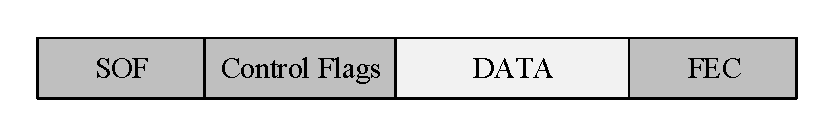
\includegraphics[width=0.75\textwidth]{chapters/chapter1/figures/frame-struct.pdf}
        \caption{常用的数据帧格式}\label{fig:1:frame-struct}
	\end{figure}
}

传输内容结构化,也是时间隐通道增强鲁棒性的常用方法。如图\nref{fig:1:frame-struct},类似IP数据包的数据帧格式,结构化数据通常包括起始标志、负载数据、辅助标记及校验信息几个部分。通过数据帧划分,有效保证了数据完整性,并且在添加了前向纠错信息后,能够纠正一定程度的传输错误。\nupcite{LIANG2018144}

%这些方法,对应用场景的限制及不足
在VoLTE场景中,对于基于主动丢包方式构造时间隐通道,对鲁棒性影响最大的是噪声中的丢包事件。为保证传输隐蔽性,主动丢弃的数据包数量要远少于网络噪声产生的丢包,导致信噪比极低。以上鲁棒性方法的前提,是接收结果中只有少量错误需要纠正。而通过主动丢包的方式构建的时间隐通道,需要由噪声中分辨出有效信息,简单的鲁棒性策略无法实现该目标,需要设计多维度的鲁棒性方法。

\subsection{时间隐通道检测方法}
\label{sec:intro:background:detect}

%检测时间隐通道,通常从哪几个要素方面进行考虑
不同于存储隐通道,时间隐通道对数据本身不产生影响。因此,存储隐通道检测方法中使用的数据内容核查,对时间隐通道是无效的。根据时间隐通道的构建方法,数据包顺序及发送间隔是产生变化的主要特征,也是时间隐通道检测方法的主要判别对象。为有效识别时间隐通道,需要对标准状态下的传输特征进行统计,并将结果作为检测过程的标准参照。

%检测判断,主要根据哪些因素来考量,包括分布、一致性
\subsubsection{基于分布曲线的检测方法}
基于分布曲线的检测方法,首先要获取样本的分布特征,并计算出CDF分布结果。通过对比参照曲线和样本曲线,判断曲线的偏离度,得出样本与标准参照是否为相同的结论。在比较方法上,除了对比曲线的基本趋势,结合量化评估方式计算最大偏离度也是常用模式。\nupcite{Cabuk:2004:ICT:1030083.1030108}K-S(Kolmogorov-Smirnov)检验是判断分布$F(x)$及$G(x)$差异的常用方式,首先统计$F(x)$及$G(x)$在相同$x$下差值绝对值的下界,并用下界值代表样本与参照之间的差异。除了K-S检验外,{Welch's\ \ t检验}也是常用的分布差异判别方法。

\insertEquation{
    \begin{equation}
    \label{equ:1:entropy}
		H(X)\ =\ -\sum_{x=i}\ p(x) \times \log(p(x))
    \end{equation}
}

\subsubsection{基于熵的检测方法}
在信息论中,熵代表了每条消息蕴含信息的多少。在时间隐通道检测中,熵反映了统计对象的离散程度。对于参照分布和样本分布来说,通过公式(\nref{equ:1:entropy})计算基于信息学的熵值,或者计算K-L(Kullback-Leibler)条件熵,可以判断样本与参照的变化程度。\nupcite{Gianvecchio:2007:DCT:1315245.1315284}与基于分布曲线检测方法不同,信息学熵值及K-L条件熵的计算对象为PMF(Probability Mass Function),也就是概率质量函数。通过判断熵值大小,判定分布一致性,在时间隐通道检测中被证明是有效可行的。\nupcite{5590253}

%在该场景中,主要通过丢包的方法构建时间隐通道,所有,在现有的常用检测方法的基础上,还要对丢包的特征进行分析
\subsubsection{面向基于主动丢包的时间隐通道检测方法}
传统的时间隐通道检测方法,聚焦于IPD分布的一致性检测,对传输过程中的丢包特征不予判别。因此现有的检测方法,无法充分证明基于主动丢包的时间隐通道具有足够的隐蔽性。基于VoLTE场景下的丢包特征,结合对应的一致性判别方法,建立有效的隐通道检测方法,从而充分证明主动丢包时间隐通道的抗检测能力。
